\chapter{Learning a Neural Code for Estimating Binocular Disparity}
\ifpdf
    \graphicspath{{chapter1/chapter1-figs/PNG/}{chapter1/chapter1-figs/PDF/}{chapter1/chapter1-figs/}}
\else
    \graphicspath{{chapter1/chapter1-figs/EPS/}{chapter1/chapter1-figs/}}
\fi

\newcommand{\runningTitle}{Learning a code for binocular disparity}
\markboth{\MakeUppercase{\thechapter. \runningTitle }}{\thechapter. \runningTitle}

% To do:
% [done] fix equations 
% [ ] replace citations
% [ ] include figures
% [ ] replace references to figures, etc...
% [ ] double check equations
% [ ] rewrite

\section{Introduction}

% Binocular simple cells and complex cells
As we have seen, binocular disparity is a powerful cue to depth estimation. Neural recordings suggest that binocular neurons in primary visual cortex (V1) initially support this ability. In particular, binocular simple cells in V1 have different receptive fields in the left and right eyes, endowing them with the capability of encoding different binocular disparities. Moreover, binocular complex cells in V1 respond selectively to particular binocular disparities, and have therefore been suggested to act as disparity detectors. 

% Computation, energy model
The computation carried out in V1 has been described by a subunit model encompassing both types of binocular neurons. The activity of binocular simple cells is modelled as linear filtering of the binocular images, followed by a rectifying non-linearity. The activity of simple cells with similar interocular disparity between their receptive fields is then combined onto a complex cell via summation. This model is known as the disparity energy model and provides a basic account of the activity of simple and complex cells \cite{Ohzawa:1990cq}. 

% Unexplained observations
However, a variety of observations are not explained by the energy model. Notably, while most binocular complex cells respond less vigourously to anticorrelated stereograms (when compared to correlated stimuli), the energy model does not reproduce this effect \cite{Cumming:1997ve}. Thus, a number of modifications based on energy model have been subsequently proposed, mostly relying on modifying the connectivity of the model or including additional non-linearities \cite{Lippert:2001fk,Read:2002kx,Haefner:2008jg}. 

% Problems with this approach
While analyzing the computational properties of these models can lead to valuable insights, their development is usually guided towards explaining neural recordings. That is, the models are hand-engineered to fit particular properties of neural responses, leaving aside the computational goal and the properties of the environment. For instance, a combination of non-linearities may reproduce a particular property of a disparity selective complex cell, but does it perform a useful computation to extract depth information from the environment? One can best answer this question by optimizing models considering the computation that V1 is thought to perform.    

% Introduce convolutional nets, deep learning
Artificial neural networks are attractive tools for this purpose - they have been extremely successful in solving complex perception and control problems \cite{NIPS2012_4824,Mnih:2015fo}, and are based on simplified versions of neurons (akin to those used in the classical energy models). Moreover, their architecture shares basic principles with the human brain, such as a densely connected networks of neurons and hierarchical structure. For instance, it has been already shown that the receptive fields developed by the first layers of such networks resemble those found in primary visual cortex \cite{NIPS2012_4824} and those that maximize efficient encoding \cite{Olshausen:1996dt}. Additionally, the representations of objects learned by these networks approximate those found in macaque and human inferotemporal (IT) cortex \cite{Khaligh-Razavi:2014yr,Cadieu:2014fk,Yamins:2014tc,Yamins:2016bh}.

% Then relate back to disparity
Given that similarities exist between these networks and the brain, particularly in early visual processing, it is interesting to ask whether these networks can be used to investigate less known encoding mechanisms in the brain. Here we investigated how a feedforward neural network computes binocular disparity based on naturalistic stereoscopic pairs. We show that a simple network trained to discriminate disparity sign on natural images solves the task using encoding mechanisms that closely agree with physiological recordings from V1. First, the binocular receptive fields developed by the model are similar to those of binocular simple cells. Second, the response properties of disparity detectors agree with those of binocular complex cells, in that their tuning for disparity in anticorrelated stereograms is inverted and attenuated when compared to correlated stereograms. We show that the presence of impossible stimuli at a given disparity causes the respective disparity detector to be suppressed, as if the network eliminates this disparity from the set of possible solutions. Moreover, we show that the network explains a range of psychophysical observations. Finally, we summarize the model in a simple equation and demonstrate that, under mild simplifications, the computes an optimal estimate of the likelihood function for binocular disparity. Our findings provide a simple and comprehensive explanation of how disparity selectivity may arise in the brain.

\clearpage
\section{Estimating disparity using artificial neural networks}

All procedures were implemented using Python. Image generation and processing were performed using standard packages for numerical and scientific computing. The convolutional network was implemented using Theano \cite{bergstra-proc-scipy-2010}, a library for efficient optimization and evaluation of mathematical expressions.

\subsection{Natural image stereoscopic pairs}

We generated naturalistic stereoscopic images using 100 light-field photographs extracted from the Light Field Saliency Database \cite{6909755}. From each acquisition in this dataset we extracted a series of images focused at different points in depth and a depth map. Each RGB image (1080-by-1080 pixels) was converted to gray-scale values and down-sampled at the resolution of the corresponding depth map (328-by-328 pixels). We rendered stereoscopic pairs by shifting the pixels of the original image by an amount proportional to the depth value, and setting the maximum shift to 10 pixels. Pixels that were revealed behind occluded regions (by displacing image features in depth) were filled using linear interpolation.
This method produced 200 stereo pairs. From these images we extracted 38,000 different pairs of smaller image patches (30-by-30 pixels). To ensure accurate disparity information, we excluded image patches with low variance of pixel intensity (gray level s.d. threshold = 20) and patches for which interpolation had been used for more that 5 \% of the pixels. All image patches were finally scaled so that pixel values were contained in the interval between –1 and 1, and randomly divided into training and test sets, as described below.
We did not use standard two frame stereo datasets (e.g. Middlebury datasets) given that these contain a large range of disparities, making it difficult to obtain sufficient training sets for a given set of disparity values. We restricted the model to work on a small number of individual disparities for which we could provide training data. Rendering stereo pairs from the corresponding depth map, as described above, allowed us to generate images with arbitrary disparity range, and therefore increase the number of class exemplars available to train the model.

\subsection{Model architecture}

We used a simple convolutional neural network that comprised (i) an input layer, (ii) a convolutional-pooling layer and (iii) an output logistic regression layer (Fig. \ref{fig:ModelArch}). In convolutional layers, the input is convolved with a series of filters - equivalent to different receptive fields - followed by a rectifying non-linearity, each producing one activity map. By analogy to simple cells, we refer to units in this layer as simple units. The use of convolution means that each filter is applied at all different locations of the input space. This significantly reduces the number of parameters that need to be learned (i.e., we do not parameterize all possible pair-wise connections between layers) and allows the network to extract a given image feature at all different positions of the image. Simple unit activity is then combined by neurons in the output layer. Once again by analogy, we refer to these neurons as complex units.
Inputs were image patches (30x30x2 pixels; the last dimension carrying the left and right images) extracted from stereoscopic images. In the convolutional layer, binocular inputs are passed through 28 binocular filters (19x19x2 pixels) producing 28 activity maps (12x12 pixels). This resulted in 4,032 units (28 maps of dimensions 12x12 pixels) forming 2,911,104 connections to the input layer (4,032x19x19x2 pixels). Since this mapping is convolutional, this required that 20,244 parameters were learnt for this layer (28 filters of dimensions 19x19x2 plus 28 bias terms). We chose units with rectified linear activation functions since a rectifying non-linearity is biologically plausible and often necessary to model neurophysiological data \cite{Adelson:1985ov,Movshon:1978dq}. More formally, the activity $a$ of unit $j$ in the $k^{th}$ convolutional map was thus given by:

\begin{equation}
  a_j^{(k)}=(w^{(k)} x_j+b_j^{(k)} )_+
\end{equation}

where $w^{(k)}$ is the 19x19x2 dimensional binocular filter of the $k^{th}$ convolutional map, $x_j$ is the 19x19x2 binocular image captured by the $j^{th}$ unit, $b_j$ is a bias term and $(.)+$ denotes a linear rectification non-linearity (ReLU). Parameterizing the left and right images separately, the activity $a_j^k$ can be alternatively written as:

\begin{equation}
  a_j^{(k)}=(w^{(Lk)} x_j^L+w^{(Rk)} x_j^R+b_j^{(k)} )_+
\end{equation}

where $w^{(Lk)}$ and $w^{(Rk)}$ represent the $k^{th}$ filter applied to left and right images (i.e. left and right receptive fields), while $x_j^L$ and $x_j^R$ represent the left and right input images captured by the receptive field of unit $j$.
The convolutional layer was followed by a max-pooling layer that down-sampled each activity map by a factor of two, producing 28 maps of dimensions 6-by-6 pixels. Finally, a logistic regression layer (1,008 connections; 36 per feature map, resulting in 1,010 parameters including the bias terms) mapped the activities in the pooling layer to two output decision units. The vector of output activities r was thus obtained by mapping the vector of activities in the pooling layer a via the weight matrix $W$ and adding the bias terms $b$, followed by a $softmax$ operation:

\begin{equation}
  r=softmax(Wa+b)
\end{equation}

The predicted class was taken to be the one corresponding to the unit with highest activity. For N-way classification, the architecture of the model was identical except for the number of output units of the model.

\begin{figure}[!h]
  \centering
  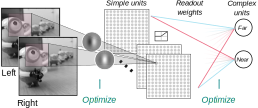
\includegraphics[width=10cm,keepaspectratio]{chapter1/chapter1-figs/ModelArchitecture.png}
  \caption[Model architecture.]{Model architecture. The left and right images are passed through a set of simple units with unconstrained preferred disparity, and their activities are readout by a set of complex units. The activity of simple units is given by the dot product between the binocular images and the corresponding receptive fields, followed by a rectified linear non-linearity. These activities are then combined onto two complex cells: one that prefers near disparities, and one that prefers far disparities. We optimized the receptive fields and the corresponding readout weights to perform near vs far depth discrimination on stereoscopic natural images.}
  \label{fig:ModelArch}
\end{figure}


\subsection{Training procedure}

The input stereo pairs were first randomly divided into training- (70\%, 26,600 pairs), validation- (15\%, 5,700 pairs) and test- (15\%, 5,700 pairs) sets. No patches were simultaneously present in the training, validation and test sets. To optimize the network, only the training and validation sets were used. We initialized the weights of the convolutional layer as Gabor filters with no differences between the left and right images. Therefore, initialization provided no disparity selectivity. With x and y indexing the coordinates in pixels with respect to the centre of each filter, the left and right monocular filters $W^L$ and $W^R$ of the $j^{th}$ unit were initialized as

\begin{equation} 
w_j^L =w_j^R = e^{(-((x'^2+ y'^2))/(2 \sigma^2 ))}  cos⁡(2 \pi f x'+\phi)
\end{equation}

where $f=0.1/pixel$, $\sigma=3 pixel$, $x'=xcos(\theta)+ysin(\theta)$, $y'=-xsin(\theta)+ycos(\theta)$, $\theta=\pi / 2 radians$, and $\phi$ is the phase of the cosine term of each unit, which was equally spaced between $0$ and $\pi$. The bias terms of these neurons were initialized to zero. In the logistic regression layer, the weights and bias terms were all initialized to zero. 

The network was trained using mini-batch gradient descent with each batch comprising 100 examples (50 examples of each class). For each batch, we computed the derivative of the loss function with respect to parameters of the model via back-propagation, and adjusted the model parameters for the next iteration according to the update rule

\begin{equation}
w_{i+1}=w_i - \alpha \big( \partial L / \partial w \big)_{D_i }
\end{equation}

where α is the learning rate, and $ \big( \partial L / \partial w \big)_{D_i}$ is the average over the batch $D_i$ of the derivative of the loss function with respect to $w$, evaluated at $w_i$. The learning rate $\alpha$ was constant and equal to 0.001.
After evaluating all the batches once - completing one epoch - we tested the model using the validation image dataset. We repeated this process for a maximum of 1,000 epochs. Initially, the maximum number of iterations allowed without improvement was set to 10,000. To allow exhaustive optimization, this limit was increased by a factor of 2 every time there was an improvement of 0.5 \% in performance as tested in the validation set.

\subsection{Evaluation}

We tested the model using both natural and synthetic images. For natural images, we tested the model using 5,700 held-out patches on the test image dataset (i.e. these exemplars were not used for training or validating the model). For comparison with neurophysiological observations, we also tested our model using random-dot stereogram patches. This test set consisted of 6,000 randomly generated stereograms containing a mixture of dark and bright dots on a gray background (dot size = 1 pixel; dot density = 50\%).

% this will probably go elsewhere
For comparison with psychophysical tasks, we also tested the model with large random-dot stereograms (240-by-240 pixels). These stereograms could contain bright dots, dark dots (single polarity cases) or a mixture of both (mixed polarity case) on a uniform mid-gray background. The dot size was set to 8 pixels and the dot density was set to approximately 15\%. No occlusion between the dots was allowed. The step disparity was set to 2 pixels. Disparity noise sampled from a Gaussian distribution (s.d.=8 pixels) was added to increase difficulty.

\subsection{Step-edge depth discrimination and depth-sign maps}
% this will probably go elsewhere
In its original form, the model takes a 30-by-30 input image patch and produces a binary output corresponding to the predicted disparity (near or far). Once trained, however, convolutional neural networks can be applied to higher dimensional inputs, without requiring any changes in the parameters of convolutional layers. We took advantage of this convenience to test the model with larger binocular inputs. The only required modification to the model happened in the readout layer, where we applied the mean read-out weight for each neural map to each unit in an element-wise manner. That resulted in two output activity maps - one for near disparities (near map), and another one for far disparities (far map). More formally, the vector of activities in the $j^{th}$ output map was defined as:

\begin{equation}
  a_{out}^{(j)}=\sum_{k=1}^{28} a_{conv}^{(k)}  \hat{w}_{out}^{(kj)}+b^{(j)}
\end{equation}

where $a_{conv}^{(k)}$ is the vector of activities in the $k^{th}$ convolutional map, $\hat{w}_{out}^{(kj)}$ is the mean readout weight between the $k^{th}$ convolutional map and the $j^{th}$ output unit, and $b^{(j)}$ is the vector of bias terms of the $j^{th}$ output unit. Finally, we combined the two output maps by element-wise subtracting the activities of the near map from the far map, so that positive values reflect higher near activity, while negative values reflect higher far activity.


\subsection{Modelling binocular receptive fields}

The receptive fields of simple units in our neural network were not constrained to develop a particular structure (i.e. Gabor functions) during optimization - they could in principle develop any kind of morphology. We therefore started by assessing whether the receptive field structure mirrored that found in simple units in primary visual cortex. In particular, we set out to test (i) if the receptive fields were well approximated by Gabor functions, and (ii) what kind of encoding mechanism they develop - i.e. position, phase or hybrid encoding.

We started by assessing whether the receptive fields were well approximated by Gabor functions. To reduce the number of free-parameters, we examined the horizontal cross-section of the receptive field, and fitted a 1-dimensional Gabor function,

\begin{equation}
  W= A \times e^{(-(x-x_0)^2/2\sigma^2}  cos⁡(2 \pi f(x-x_0)+\phi).
\end{equation}

We used a two-stage procedure for optimization. First, we ran a coarse grid-search to find a good initial guess for the parameters, whereby the combination of parameters with lowest sum of squared errors was selected. Then, taking the grid-search estimates as initial guesses, we estimated the final parameters using bound constrained minimization. The constrained parameters were the amplitude ($0<A<+\infty$), the center of the envelope ($min(x)<x_0<max(x)$), the phase ($-\pi<\phi<\pi$) and the frequency, which was constrained to an interval of $\pm10 \%$ around the peak of the Fourier transform of the receptive field profile. To assess whether disparity was encoded via position and/or phase shifts, we subtracted the position/phase parameters between the left and right receptive fields. The phase parameter was subsequently wrapped to $[-\pi, \pi]$.


\subsection{Estimating correlated vs anticorrelated amplitude ratios}

Complex cells in V1 respond more vigorously to correlated (cRDS) than anticorrelated stereograms (aRDS) \cite{Cumming:1997ve}. We examined whether the degree of attenuation observed in our model units was compatible with electrophysiological data. Attenuation is commonly assessed by modelling tuning curves for aRDS and cRDS, and then evaluating the ratio between the corresponding amplitudes \cite{Cumming:1997ve,Samonds:2013cs}. Therefore, we modelled the tuning curves using Gabor functions (similar to those used to model the binocular receptive fields) and computed the ratio between the amplitude parameter for correlated and anticorrelated stimuli. We started by generating disparity tuning curves for each complex unit by computing the activity elicited by correlated or anticorrelated random-dot stereograms (50 \% dot density) with disparities ranging from -20 to 20 pixels (100 trials per disparity). To avoid relying on a single fit per complex unit, we used bootstrapping to generate 5000 resampled tuning curves, and we fitted a Gabor to each sample. Based on these parameters, we computed the respective amplitude ratios by dividing the amplitudes for aRDS by the amplitudes for cRDS. We finally arrived at a distribution of amplitude ratios by pooling the data across complex units.

\subsection{Computing optimal stimuli}\label{ssec:OptStim}

To confirm that the model was well tuned to extract physical binocular disparities, we computed the input images that best activate the complex units of our model. The intuition is that we can visualize which inputs are most efficient in driving a given complex unit, and thereafter evaluate whether the input is sensible. The objective function is therefore the activity of a given complex unit, which we want to maximize. Equivalently, for an output unit $j$, we minimized the negative of its input:

\begin{equation}
  L_j = - \big( \mathbf{W}_j \mathbf{a} + b_j \big) 
  \label{eq:OptLoss}
\end{equation}

where $\mathbf{a}$ is the vector of simple unit activities, $W_j$ is the readout weight matrix for the $j^{th}$ complex unit, and $b_j$ is the respective bias term. The goal is thus to find an input image that minimizes $L_j$. We did this via gradient descent: we started with a random noise input image, $\mathbf{S}_0$, computed the gradient of the loss function with respect to the input image, and adjusted the latter according to the update rule:

\begin{equation}
  S_{i+1} = S_i - \alpha \frac{\partial L}{\partial S}
\end{equation}

where $\alpha$ is the step size (empirically set to 1). We limited the number of iteration to 100 as this was enough to ensure that optimization reached a stable solution (i.e. the correlation between the stimulus in two consecutive iterations saturated at 1). This iterative method produced the input stereo pair that best activated the complex units of the model.

\clearpage
\section{Neurophysiological correlates} 
% - Simple cell receptive fields
% - Complex cell properties
% - Compound grating
% - Optimized stimuli
% - ?implementation in the brain (spiking network)?

Our primary goal was to train a neural network on a simple disparity discrimination task on binocular natural images, and examine if the properties developed by the model agree with those observed in neural recordings. Briefly, the neural network consisted of a layer of simple units, followed by a layer of complex units. The parameters of the model (i.e. the binocular receptive fields and corresponding readout weights) were optimized for a near vs. far depth discrimination task via error back-propagation using binocular patches sampled from natural images. Following optimization, the network was able to classify depth in novel, held-out images with high accuracy (A=99.23\%). Having confirmation that the training procedure was successful, I next compared the properties of the model to those of simple and complex cells in V1. 

First, I examined the receptive fields of simple units (Fig. \ref{fig:BinocularRFs}). They were well approximated by Gabor functions (Fig \ref{fig:BinocularRFs}A; mean $R^2=0.95$, $s.d.=0.049$) and presented both position and phase offets (Fig. \ref{fig:BinocularRFs}B) consistent with V1 simple cells \cite{Ohzawa:1986af,DeAngelis:1991mb,Tsao:2003pi}. Only 3 out of the 28 types of receptive field responded to position offsets without phase offsets, and removing units with near-zero phase disparities (i.e., the seven units within ±π/4) did not significantly affect the network’s decoding performance (p=.76), suggesting no privileged role for position disparities.

\begin{figure}[!h]
  \centering
  \includegraphics[width=14cm,keepaspectratio]{chapter1/chapter1-figs/BinocularRFs.png}
  \caption[Binocular receptive fields developed by the model.]{Binocular receptive fields developed by the model. A, Left: binocular receptive fields developed by the model. Right: 1-dimensional receptive field profile for a simple unit (black), and a simple cell in cat primary visual cortex \cite{DeAngelis:1991mb}. B, Summary of position and phase shifts for the population of units in the model.}
  \label{fig:BinocularRFs}
\end{figure}

Next, I examined the properties of complex units. I started by testing if they were selective for depth in random-dot stimuli typically used in the laboratory. Although the optimization was based on natural images, the performance was excellent ($A=99.93 \%$; $CI_{95\%} =99.87\%, 99.98\%$) for correlated random-dot stereograms (cRDS). I then tested if complex units were also selective anticorrelated stimuli (aRDS), in which a dark dot in one eye matches a bright dot in the other. V1 neurons respond to the disparities in these stimuli, however their disparity tuning function is inverted \cite{Cumming:1997ve}. Accordingly, the network systematically mis-predicted the stimulus depth ($A=8.83\%$; $CI_{95\%}=7.62\%, 9.03\%$), albeit with a lower accuracy then would be expected by simple inversion of the response. 

This indicated that complex units were less selective for anticorrelated stimuli. To test this, we computed complex unit tuning curves for disparity in correlated and anticorrelated stereograms (Fig. \ref{fig:cRDSaRDS}A). Consistent with complex cells in V1 \cite{Cumming:1997ve,Samonds:2013cs}, we found inverted and attenuated activity in response to anticorrelated stereograms. We computed bootstrapped estimates of the ratio between responses amplitude to aRDS vs. cRDS, we found striking similarities to the ratio exhibited by V1 neurons \cite{Cumming:1997ve,Samonds:2013cs} (Fig. \ref{fig:cRDSaRDS}B). The inversion in the tuning curve results from an increase in suppressive input to the preferred complex unit (Fig. \ref{fig:cRDSaRDS}C).

\begin{figure}[!h]
  \centering
  \includegraphics{chapter1/chapter1-figs/cRDS_aRDS.png}
  \caption[Response to random-dot stereograms.]{Response to random-dot stereograms. A, Disparity tuning curve for the near complex unit in response to cRDS and aRDS; the shaded area shows 95\% CIs of the mean (5000 resamples). B, Distribution of amplitude ratios for cRDS vs. aRDS for the model (bar histogram; 5000 resamples per complex unit), and disparity selective cells in macaque V1: Red series, 72 neurons \cite{Cumming:1997ve}; orange series, 103 neurons \cite{Samonds2013}. C, Summary of excitatory (magenta elements) and suppressive (cyan elements) drive to the near complex unit for correlated and anti-correlated stereograms. Error bars (hardly visible) represent CI95\%. of the mean}
  \label{fig:cRDSaRDS}
\end{figure}

% write a bit more here...
To confirm that these observations were not specific to binary classification, we also trained a network to perform $n$-way classification. The only change required to the model was an increase in the number of output complex units (from two to $n$). In particular, we optimized a model for 7- and 11-way classification. In these cases, the complex units of the model also display inversion and attenuation for anticorrelated random-dot stereograms, with comparable but more variable amplitude ratios (Figure \ref{fig:Nway}).

\begin{figure}
  \centering
  \includegraphics[width=13cm,keepaspectratio]{chapter1/chapter1-figs/Nway.png}
  \caption[N-way classification.]{N-way classification. Disparity tuning curves of output units for 7-way (A) and 11-way (B) classification. Inversion and attenuation can be observed in the majority of the units. There is considerable variability in the degree of attenuation across units, consistent with neurophysiological observations. Bootstrapped estimates of the mean amplitude ratio are shown on the right of each panel. Bar graphs depict amplitude ratio (aRDS/cRDS) calculated based on peak-to-peak differences (mean and $68\%$ confidence intervals obtained via bootstrapping, 5000 resamples per output unit). A bias towards values below unity is evident.}
  \label{fig:Nway}
\end{figure}

So far, our results indicate that complex units are optimized for valid binocular disparities - disparities that correspond to the physical translation of an object. To investigate this further, we borrowed a clever idea from neurophysiology experiments \cite{Haefner:2008jg}. Consider an image of a fronto-parallel surface with a particular spectral content. A physical horizontal translation of the surface causes a different phase shift in the individual spatial frequency components. The resulting phase shifts are related to the horizontal translation by means of the spatial frequency, $\Delta \phi= \Delta x f$. A combination of phase shifts that does not respect this relationship can thus be considered as non-physical. Physical and non-physical disparities can be however be simulated using compound gratings. These stimuli consist of a sum of two gratings with different spatial frequencies, and whose phase can be independently manipulated. Therefore, we can examine whether the responses of complex cells are optimized for physical disparities.

To facilitate comparison to neurophysiology data, we used compound gratings comprising two different spatial frequencies differing by a factor of two. The phase shifts that correspond to a physical disparity are thus given by $ \Delta \phi_1 = 2 \Delta \phi_2 $. If complex cells are indeed optimized for detecting binocular disparities, they should dedicate their maximum dynamic range (i.e. they should be maximally excited and suppressed) in response to phase shifts that respect the physical constraint. Neurophysiologists have shown that this is indeed the case for many complex cells in macaque primary visual cortex \cite{Haefner:2008jg} (Fig. \ref{fig:CompGrating}B). This is not the case for complex cells as defined by the classical disparity energy model. The complex units in our model, however, produce their maximum and minimum response along the physical disparity line (Fig. \ref{fig:CompGrating}A), indicating that they are optimized to extract physical disparities.

\begin{figure}[!h]
  \centering
  \includegraphics[width=14cm, keepaspectratio]{chapter1/chapter1-figs/CompoundGrating.png}
  \caption[Model response to compound gratings.]{Model response to a compound gratings. A, Response of one complex unit of the model. B, Corresponding raw (left) and smoothed (right) data for a complex cell in macaque V1 \cite{Haefner:2008jg}.}
  \label{fig:CompGrating}
\end{figure}

% segue to optimal stimuli
We devised yet another test to confirm that complex units were well optimized for extracting physical disparities. In particular, we sought to visualize the stimuli that best activated the complex units. We first computed the response of a given complex unit to a noise image pair. Then, we computed the gradient of the response with respect to the pixels of the input images, and iteratively adjusted the pixel values so as to maximize the response (see \ref{ssec:OptStim}). This optimization procedure produced stimuli that resembled Gabor patches with similar structure but horizontally translated between the eyes, in the direction consistent with the preferred disparity of the complex unit. This is consistent with detecting disparities caused by physical, positional offsets. The structure of the Gabor patches was however very similar across the eyes, indicating that stimuli with non-physical (i.e. phase) disparities are not ideal to activate the complex units of the model.

\begin{figure}[!h]
  \centering
  \includegraphics{chapter1/chapter1-figs/OptimalStimuli.png}
  \caption[Computing the optimal stimulus for a complex unit in the model.]{Computing the optimal stimulus for a complex unit in the model. Starting with noise inputs, we compute the activity of the complex unit of interest (here $y_0$ for the \textit{near} unit). We wish to maximize this activity, or alternatively minimize its negative, $L_0$ (Equation \ref{eq:OptLoss}). To do that, we compute the gradient with respect to the input images, $\frac{\partial L_0}{\partial S}$, and adjust the inputs via gradient descent. Finally, we iterated through this procedure.}
  \label{fig:OptStim}
\end{figure}

Our complex units account for many properties of V1 complex cells. But how does this arise? To answer this question, we need understand how the activity of simple units is combined onto complex units. We found that a simple rule governs the relationship between readout weights and receptive fields: weights are proportional to the value of the cross-correlogram between the (left and right) receptive fields (R=0.89; p<.001) (Fig \ref{fig:WR}). The intuition (which we later formalize) is that receptive fields that capture a positive correlation at a given disparity δi (i.e. the lag of the cross-correlogram) should be readout by a complex unit with preferred disparity δi using a positive (i.e. excitatory) weight. Conversely, if the simple unit captures a negative correlation at disparity δi, the complex unit should readout its activity using a negative (i.e. suppressive) weight. 

\input{chapter1/chapter1-figs/FigWR.tex}

Consistent with our model, convergence of excitatory and suppressive inputs with different tuning properties onto individual complex cells is observed in neurophysiology \cite{Tanabe:2011pt}. Moreover, neural recordings indicate that the particular feedforward arrangement followed by our network is plausible \cite{Tanabe:2014ud}. In particular, suppression is only briefly delayed in relation to excitation (approximately 7ms) \cite{Tanabe:2014ud}, suggesting feedforward inhibition as a likely mechanism.

In sum, we have shown that the model develops physiologically plausible receptive fields, and reproduces responses of V1 complex cells to correlated and anticorrelated random-dot stereograms. Like many complex cells in V1, complex units in our model are well tuned to physical disparities. Importantly, these properties developed through optimization for computing binocular disparity from naturalistic stereo pairs. 

\clearpage
\section{Perceptual correlates}

% The influence of interocular contrast differences
Given the good agreement between our model and the properties of simple and complex cells in V1, we wondered whether we could account for psychophysical observations pertaining to early disparity processing. In particular, we wondered whether the model could qualitatively reproduce data from experimental tests pertaining to how interocular contrast differences affect binocular processing. 

A seminal study by Smallman \& McKee proposed that the visual system uses a constant contrast ratio constraint for binocular matching \cite{Smallman:1995fk}. By manipulating interocular contrast in a competitive matching, the authors found that the contrast required for matching features with different contrasts grows linearly with contrast magnitude (Fig. \ref{fig:ContrastRatio}, left). We tested whether this relationship held for our model. In particular, we systematically varied the interocular contrast while examining the performance of the model. As in the human visual system, we found a linear dependency between the contrast required for matching and contrast magnitude (Fig. \ref{fig:ContrastRatio}, right). Moreover, the slope of the line was very close to unity (0.99), in good agreement with psychophysical measurements \cite{Smallman:1995fk}.
% might need to give more details here (number of trials, 70% correct, etc)

\begin{figure}[!h]
  \centering
  \includegraphics[width=10cm, keepaspectratio]{chapter1/chapter1-figs/contrast-ratio.png}
  \caption[Contrast ratio constraint.]{The contrast ratio constraint. Left, psychophysical measurement of contrast in the right image (ordinate) necessary to match a higher contrast feature in the left image (abcissa). Different colors represent data from three subjects, and lines represent linear regression in log-log space. The data is reproduced from \cite{Smallman:1995fk}. Right, interocular contrast relationship for our model. Black dots represent data for individual contrast levels, and the gray line represents linear regression in log-log space. Regression lines from \cite{Smallman:1995fk} are plotted in color for comparison.}
  \label{fig:ContrastRatio}
\end{figure}

These psychophysical results suggest that the visual system explores differences interocular contrast to solve stereo correspondence. Two main computational mechanisms have been proposed to underly this process - correlation and matching. Interocular correlation simply computes the correlation between the half images at different disparities, and the disparity at which the highest correlation occurs is selected as the target disparity. When the half images are anticorrelated, the interocular cross-correlation is reversed, and the wrong disparity is systematically predicted. Matching computations, however, seek to find correspondence only between similar features (e.g. with similar contrast).

The visual system does not seem to strictly follow any of these rules. When interocular contrast is reversed, human observers can under some circumstances perceive the opposite depth significantly below chance. A correlation based mechanism predicts systematically the opposite response, while matching predicts performance at chance level. To bridge this gap, alternatives have been suggested based on independent matching and correlation channels \cite{Doi:2011ku,Fujita:2016uq} or modifications to the disparity energy model (Henrikssen, PLoS Comp Biol). We wondered whether our model could account for this characteristic of perception. Similar to psychophysical studies \cite{Doi:2011ku}, we computed the performance of the model as the proportion of correlated dots in a random-dot stereograms was varied. We found that our model performed in qualitative agreement with the psychophysical data. In particular, the model does not follow the behaviour predicted by correlation or matching (Fig. \ref{fig:PropCorrelated}). When the same number of correlated and anticorrelated dots are present, our model performs above chance level. However, when the stimulus in fully anticorrelated, the model performs below chance level - but not perfectly. Therefore, our model deviates from correlation and matching in the same direction that human performance does. 

\begin{figure}
  \centering
  \includegraphics[width=6cm, keepaspectratio]{chapter1/chapter1-figs/prop-correlated.png}
  \caption[Model performance as a function of binocular correlation.]{Model performance as a function of binocular correlation. Computational mechanisms based on correlation and matching respond differently to variations in binocular correlation. Correlation mechanisms perform at chance level when the stimulus features equal number of correlated and anti-correlated dots, and predicts perfectly the wrong disparity when stimuli consist solely of anti-correlated features (blue curve). Matching mechanisms, conversely, reach chance level only when the stimulus is perfectly anti-correlated, and perform above chance otherwise (green curve). Our model does not follow strictly either of these mechanisms (black elements).}
  \label{fig:PropCorrelated}
\end{figure}

It is thus clear that the visual system does not ignore anti-correlation. One possibility supported by our model is that anti-correlation is actively sensed to rule out incorrect disparities. In other words, seeing depth should be easier when there is more potential for anticorrelation at the incorrect disparity. This logic naturally explains a long-standing puzzle from the psychophysical literature \cite{Harris1995,Read:2011ix} that demonstrated better depth discrimination with stimuli consisting of dark and bright dots (mixed polarity; Fig. \ref{fig:Polarity}A, top) compared to only dark or only bright dots (single polarity; Fig. \ref{fig:Polarity}A, bottom). Indeed, we found that our model performed better with mixed as opposed to single polarity stereograms (Fig. \ref{fig:Polarity}B), and the efficiency ratio between these conditions qualitatively agrees with human psychophysical efficiency \cite{Harris1995}.

\begin{figure}
  \centering
  \includegraphics{chapter1/chapter1-figs/polarity.png}
  \caption[Model performance depends on contrast polarity.]{Model performance depends on contrast polarity. A, Illustration of mixed vs single polarity stereograms. Dots in the single polarity stereograms were either all dark, or all bright; B, Proportion of correct choices (near vs far) for mixed and single polarity stereograms (250 trials per condition). Error bars depict bootstrapped 95\% CIs (5000 resamples); C, Efficiency ratio between mixed and single polarity stimuli measured psychophysically \cite{Harris1995} and for our model. Error bars represent bootstrapped 95\% CIs (5000 resamples)}
  \label{fig:Polarity}
\end{figure}

From the previous example, it directly follows that depth perception should be hindered when anticorrelation is introduced at the correct disparity, more so than if anticorrelation is introduced elsewhere. We developed a demonstration that clearly shows this effect (Fig. \ref{fig:DemoInvert}). We started by creating a random-dot stereogram that depicts a target step-edge using only correlated dots - in this case, stereopsis is achieved easily (Fig. \ref{fig:DemoInvert}, reference). We then compared the effects of adding anticorrelated dots with the same or opposite disparity sign (Fig. \ref{fig:DemoInvert}, same vs opposite). Stereopsis can still be well achieved when anticorrelation occurs at the opposite disparity sign, but is severely hindered when anticorrelation occurs at the same disparity sign.

\begin{figure}
  \centering
  \includegraphics[width=14cm, keepaspectratio]{chapter1/chapter1-figs/DemoInvert.png}
  \caption[Perceptual impact of disparity anti-correlation.]{Demonstration of the perceptual impact of disparity anticorrelation. A, A reference step edge in depth was rendered using only correlated dots (left). Anticorrelation with the same (middle) or opposite (right) disparity sign was then added. B, Corresponding random-dot stereograms. Anticorrelation at the opposite disparity sign is less disruptive than anticorrelation at the same disparity. The effect is best visible when the stack of stereograms subtends approximately 1 degree.}
  \label{fig:DemoInvert}
\end{figure}

Monocular occlusions due to viewing geometry can also cause binocular incogruencies in contrast: due to occlusion around the edges of an object, some features are visible to one eye, but not the other. That potentially leads to features that are present exclusively in one of the half images, and therefore matching them is impossible. Psychophysical evidence shows that the brain exploits such unpaired elements to support depth perception \cite{Gillam:1988lo,Nakayama:1990fc}. We demonstrated these effect in our model using a stimulus with unpaired features around a zero-disparity square target (Fig. \ref{fig:Davinci}A, left). Because the square target was not displaced in depth, there are no binocular corresponding features that could be used to compute the depth relationship. The network was able to predict the ordinal depth structure experienced by observers viewing the stereogram (Fig. \ref{fig:Davinci}A, right). This occurs because the flanks and the central target have opposite contrast polarity, and therefore they cannot to be matched. The disparity at which that match would occur is therefore suppressed, pushing the output away from that prediction (in particular, to the opposite disparity sign).

We devised another demonstration of the same effect using the ‘wallpaper illusion’ \cite{Anderson:1994fk}, where disparity matches are ambiguous - i.e. the wallpaper pattern can be seen either nearer or farther. In this case, the disparity-sign map produced by the network did not identify a clear depth edge around the sides of the pattern (Fig. \ref{fig:Davinci}B, top). However, manipulating the background intensity introduces contrast polarity violations and biases the perceptual experience \cite{Anderson:1994fk}. Upon manipulating background intensity, the network predicted the perceptual interpretation of the stereograms (Fig. \ref{fig:Davinci}). It is the polarity constraint implemented by the network that underlies the shift in disparity-sign prediction. 

\begin{figure}
  \centering
  \includegraphics[width=10cm, keepaspectratio]{chapter1/chapter1-figs/davinci.png}
  \caption[Model performance in half-occluded regions.]{Model performance in half-occluded regions. A, Da Vinci stereopsis. Left: Illustration of half-occlusions (black flanks) produced by viewing geometry; Center: stereograms of ‘Da Vinci’ stereopsis for cross-eyed fusion; Right: and the ordinal depth predictions of our model. B, Wallpaper illusion. Top: Ambiguous wallpaper pattern. The vertical stripes in this pattern can be matched both by nasal or temporal shift - both “near” and “far” global matches are valid. Cross-eyed fusion of the stereogram allows the reader to experience alternation between the stripes appearing closer vs. farther away that the background. In this case, our model does not detect a clear depth around the edges of the pattern. Bottom: Eliminating the perceptual ambiguity by manipulating background intensity is accompanied by a shift in the performance of our model.}
  \label{fig:Davinci}
\end{figure}

\clearpage

\section{A generalized model}
% This is where theory kicks in. This section could also be called "A theoretical framework" 
% Part 1: Why use hybrid receptive fields?
% Part 2: Optimal readout - derivation
% Part 3: Results (population responses, tuning curves, transparency, ...)

So far, we have shown that a neural network optimized for computing binocular disparity in naturalistic stereoscopic pairs accounts for neurophysiological and perceptual observations. In this section, we aim to describe the neural network in a simplified form and provide interpretive insights. Our goal is to generalize the model implemented in the neural network (reducing it to simple equations), and provide theoretical arguments for why it is useful.

We start by considering the question of how binocular disparity is first encoded by simple units. Why does the brain, and our model, develops hybrid receptive fields? We approach this question using information theory, under the hypothesis that hybrid receptive fields may encode more information about stimulus disparity. We then move on to derive a generalized model based on the properties developed by the neural network.  

\subsection{Information theory and binocular receptive fields}

\subsubsection*{Individual simple units}
We sought to formalise the idea that information encoded in the responses of binocular simple units is not restricted to the preferred disparity. To do so, we computed the Shannon information $I$ between broadband stimuli $s$ with varying disparity $\delta$ and simple unit responses $R$,

\begin{equation}
  I(R, s_\delta) = \sum_i p(r_i|s_\delta) \log \frac{p(r_i|s_\delta)}{p(r_i)},
  \label{eq:ShannonInformation}
\end{equation}
 
where $r_i$ denotes the firing rate of the simple unit. The resulting information indicates how well a particular disparity is encoded in the response of the simple unit. In this demonstration, the receptive fields were parameterized as two-dimensional $(x,y)$, vertically oriented Gabor functions,

\begin{equation}
  W(x,y) = e^{((x-x_0)^2 + y^2)/2\sigma^2} \cos (2 \pi f (x-x_0) + \phi),
\end{equation}

where $\sigma$ denotes the Gaussian envelope width, $x_0$ denotes the position, $f$ the spatial frequency, and $\phi$ denotes the phase of the receptive field. To define the disparity encoded by the simple unit, we varied the phase and/or position, and kept the remaining parameters constant. Varying the position parameter introduces a simple translation in the receptive field, while varying the phase causes a change in the internal structure of the receptive field (Figure \ref{fig:DispEnc}A).

We computed the information carried by a simple cell with preferred disparity of 4 pixels defined by a \textit{(i)} position shift, \textit{(ii)} phase shift and \textit{(iii)} hybrid position/phase shift. For this simulation, the receptive field envelope, $\sigma$, was set to 5 pixels and the frequency, $f$, was set to 0.05 cycles/pixel. The stimulus set consisted of 100000 uniform noise images with disparities between -20 and 20 pixels. For all three encoding mechanisms, we observed that individual simple units convey information about non-preferred disparities (\ref{fig:DispEnc}B). This highlights that the activity of simple units selective for a particular disparity could contribute to the activity of complex units tuned to different disparities.

\begin{figure}
  \centering
  \includegraphics[width=10cm, keepaspectratio]{chapter1/chapter1-figs/EncodingInformation.png}
  \caption[Information and disparity encoding in simple cells.]{Information and disparity encoding. \textbf{A}, One dimensional illustration of disparity encoding via position, phase, or hybrid shifts. \textbf{B}, Simple cells with position, phase, or hybrid shifts encode information about non-preferred stimulus disparity.}
  \label{fig:DispEnc}
\end{figure}

\subsubsection*{Population of simple units}

In the previous section we examined information at the single unit level (i.e. how much information about stimulus disparity is encoded in simple cells). Next, we demonstrate how much information is encoded across a small population of simple units (N=5) with position, phase and hybrid disparity encoding. Although we are now working at the level of multiple simple units, equation \ref{eq:ShannonInformation} can still be used to compute the Shannon information - the difference is that the response is a vector of activities of multiple simple units, and therefore the underlying probability distributions over the responses are multidimensional. Because we are not interested in the information about individual stimulus disparities, but rather how well all disparities are encoded, we integrate over the stimulus disparity,   

\begin{equation}
  I(\mathbf{R}, \mathbf{S}) = \sum_\delta \sum_i p(\mathbf{r_i}|s_\delta) \log \frac{p(\mathbf{r_i}|s_\delta)}{\mathbf{p(r_i)}}.
  \label{eq:ShannonInformationVector}
\end{equation}

We generated populations of simple units with \textit{(i)} position shifts, \textit{(ii)} phase shifts, or \textit{(iii)} a combination of both (hybrid encoding). The Gaussian envelope width, $\sigma$, and the spatial frequency, $f$, were kept constant, and only the position $x_0$ and the phase $\phi$ parameters were allowed to vary. 

We examined information encoded under two schemes. First, we computed the information under the assumption of uniformly spaced simple units. This ensures minimal overlap between the tuning curves of the simple units, and therefore avoids redundancy (i.e. the suboptimal case where two or more units in the population have very similar tuning curves). Next, we examined information without imposing this uniform spacing, and allowed the simple units to assume random tuning profiles. We did this by generating 1000 populations for which the position and/or phase shifts (according to the encoding mechanisms under evaluation) were randomly drawn from a uniform distribution. This yielded a distribution of information values for each of the mechanisms. As expected, we observed higher information values for the uniformly distributed population (\ref{fig:DispEncPop}, horizontal lines) when compared to random populations (\ref{fig:DispEncPop}, bar graph). In both cases, we found that hybrid populations carried the most information about the disparity imposed in our stimulus set (\ref{fig:DispEncPop}). This provides a potential explanation for why simple cells in primary visual cortex present hybrid receptive fields.

\begin{figure}
  \centering
  \includegraphics{chapter1/chapter1-figs/EncodingInformationPop.png}
  \caption[Information and disparity encoding in populations of simple cells.]{Information and disparity encoding in populations of simple cells.}
  \label{fig:DispEncPop}
\end{figure}

\subsection{Derivation of a generalized model}

We will now derive a simplified, generalized model based on the properties of our neural network. We will start by making a formal link between binocular receptive fields and disparity selectivity for simple cells. This link will be useful at a later stage, when establishing a relationship between the selectivity of simple cells, and the weight with each complex cells readout simple cell activity.

\subsubsection*{Interocular RF cross-correlation and disparity selectivity}
It has been noted elsewhere that computing the cross-correlogram between the left and right receptive fields yields a very good approximation of the disparity tuning curve \cite{Ferster:1981kl,Tsao:2003pi}. Below we present a derivation that describes this relationship. We start by considering the response $r$ of binocular simple cells to a given binocular stimulus with disparity $\delta$. The binocular half images (i.e. the images captured by the left and right eyes) are horizontally translated versions of one another. Thus, the stereo pairs presented in a given trial $t$ can be defined as $\{S_t(x), S_t(x+\delta)\}$. As observed experimentally, the response of a binocular simple cell can be well described by linear spatial filtering and rectification, followed by a non-linearity \cite{Ohzawa:1990cq,Anzai:1999uq},

\begin{equation}
r = g \big( [S_t(x) W_L(x) + S_t(x+\delta) W_R(x)]_+ \big),
\end{equation}

where $W_L(x)$ and $W_R(x)$ denote the receptive fields of the simple cell for the left and right eyes, and $g$ is an expansive nonlinearity. It has been shown that this non-linearity is well described by a power law with an exponent of approximately 2, $g(x) = x^2$, for $x > 0$ \cite{Anzai:1999uq}. Based on this, we can compute a disparity tuning curve, $f(\delta)$, by averaging the response of the simple cell across a large number of trials $T$, 

\begin{IEEEeqnarray}{rCl}
f(\delta) & = & \frac{1}{T} \sum_{t=1}^T r_t \nonumber \\
& = & \frac{1}{T} \sum_{t=1}^T \Bigg( S_t(x) W_L(x) + S_t(x+\delta) W_R(x) \Bigg)^2 \nonumber \\
& = & \frac{1}{T} \sum_{t=1}^T \Bigg( (S_t(x) W_L(x))^2 + (S_t(x+\delta) W_R(x))^2 \nonumber \\
& & + \ 2 S_t(x) W_L(x) S_t(x+\delta) W_R(x) \Bigg).
\end{IEEEeqnarray}

As many others have noted \cite{Fleet1996,Anzai:1999uq,Read:2002kx,Qian:1997bu}, the first two terms are monocular and do not depend on binocular disparity - over many trials, these two terms should be a non-negative constant independent of the disparity $\delta$ of the stimulus. The disparity dependent modulation of the tuning curve is captured by the interaction term,
 
\begin{IEEEeqnarray}{rCl}
f(\delta) & = & \frac{1}{T} \sum_{t=1}^T \ 2 \ S_t(x) W_L(x) S_t(x+\delta) W_R(x).
\end{IEEEeqnarray}

This expression describes the expected response for a simple cell with receptive fields $W_L(x)$ and $W_R(x)$ to stereoscopic pairs that are translated horizontally in relation to one another by a given disparity $\delta$. Under this formulation, the response of the simple cell is proportional to the stimulus unnormalized cross-correlation, $S_t(x)S_t(x+\delta)$, weighted by the product of the left and right receptive fields, $W_L(x)W_R(x)$, known as the binocular interaction field\cite{Anzai:1999uq}. However, because the stereoscopic pairs are simply translated in relation to the position of the receptive fields, it is equivalent to compute a disparity tuning curve by applying the horizontal shift to the receptive fields, while keeping the stereoscopic images in the same horizontal position ($a(x-\delta)b(x)=a(x)b(x+\delta)$),

\begin{IEEEeqnarray}{rCl}
f(\delta) & = & \frac{1}{T} \sum_{t=1}^T \ 2 \ S_t(x) W_L(x) S_t(x) W_R(x-\delta) \\
& = & \frac{1}{T} \sum_{t=1}^T \ 2 \ S_t(x)^2 \ W_L(x) W_R(x-\delta).
\label{dtXcorr}
\end{IEEEeqnarray}

Equation \ref{dtXcorr} is convenient because it expresses the disparity tuning curve as a function of the dot product between the left and right receptive fields, translated according to the disparity $\delta$. This is by definition the cross-correlation between the left and right receptive fields $(W_L \star W_R)[\delta]$. Note that $\frac{1}{T} \sum_{t=1}^T S_t(x)^2$ is simply the average energy of the stimulus over $T$ trials, which influences the amplitude of the tuning curve (but not its morphology). Therefore,

\begin{IEEEeqnarray}{rCl}
f(\delta) & = & 2 (W_L \star W_R)(\delta) \ \frac{1}{T} \Bigg( \sum_{t=1}^T S_t(x)^2 \Bigg) \\
& = & 2 (W_L \star W_R)[\delta] \ \mathbb{E} \Big( S_t(x)^2 \Big).
\label{dtXcorrEnergy}
\end{IEEEeqnarray}

Figure \ref{fig:RespCorr} demonstrates that indeed there is a very good relationship between the response of a simulated simple unit and its interocular receptive field cross-correlogram. This relationship has been also observed for simple cells in primary visual cortex\cite{Tsao:2003pi}.

\input{chapter1/chapter1-figs/FigRespCorr.tex}

\subsubsection*{Optimal readout of simple cell activity by disparity selective complex cells}

In the previous section, we showed that the disparity tuning curve of a simple cell can be well approximated by the scaled cross-correlogram between the left and right receptive fields. We also suggested that stimulus contrast energy induces variability in the firing rate of simple cells. This high variability makes simple cells unsuitable for the detection of depth. By combining the activities of multiple simple cells, complex cells provide much better estimates of disparity. The classical disparity energy model obviates this problem by combining the outputs of four simple cells with the same preferred binocular disparity, but with their receptive field phase in quadrature \cite{Ohzawa:1990cq}. 

We now ask how could we optimally combine the activities of a population of simple cells with highly variable firing rates. Inspired by previous work on optimal sensory representations \cite{Jazayeri:2006fk}, we tackle this problem from a probabilistic viewpoint. Let us interpret the distribution of activity of a simple cell $i$ given a particular disparity $\delta$ as describing the likelihood of observing the firing rate $r_i$ given the disparity $\delta$. We assume that the response of a simple cell in individual trials is normally distributed around the mean firing rate value, which is given by the corresponding tuning curve, $f_i(\delta)$. Thus, the likelihood for a given simple cell $i$ is given by

\begin{equation}
  p(r_i | \delta) = \frac{1}{\sqrt{2 \pi \sigma_i}} e^{- \frac{(r_i-f_i(\delta))^2}{2 \sigma_i^2}}.
\end{equation}

This equation expresses the probability of observing a firing rate $r_i$ given a stimulus with disparity $\delta$. Assuming independence across a population of $N$ simple cells, we can now combine these probabilities to obtain a joint likelihood,

\begin{equation}
 L(\delta) = p(\mathbf{r} | \delta) = \prod_{i=1}^N p(r_i| \delta) .
\label{eq:JointLikelihood}
\end{equation}
 
By working in log-space, we can convert the logarithm of the product of likelihoods into a sum of logarithms of the likelihood. This is useful because we can express the computation of the likelihood as sum over the activity of many neurons, which is a biologically plausible operation. Equation \ref{eq:JointLikelihood} thus becomes

\begin{IEEEeqnarray}{rCl}
 \log L(\delta) & = & \sum_{i=1}^N \log p(r_i| \delta) \\
& = & \sum_{i=1}^N \log \Bigg( \frac{1}{\sqrt{2 \pi \sigma_i}} e^{- \frac{(r_i-f_i(\delta))^2}{2 \sigma_i^2}} \Bigg) \\
& = & \sum_{i=1}^N -\frac{(r_i-f_i(\delta))^2}{2 \sigma_i^2} - \log \big(\sqrt{2 \pi \sigma_i}) \\ 
& = & \sum_{i=1}^N \frac{r_i f_i(\delta)}{\sigma_i^2} - \frac{1}{2} \Bigg( \frac{r_i^2}{\sigma_i^2} - \frac{f_i(\delta)^2}{\sigma_i^2} - \log \big(2 \pi \sigma_i) \Bigg).
\label{eq:LogLikelihoodDisp}
\end{IEEEeqnarray}

The second term in equation \ref{eq:LogLikelihoodDisp} can be ignored if we assume that the tuning curves of the population of simple cells cover homogeneously the disparities of interest, and thus $ \sum_{i=1}^N f_i(\delta)^2 = constant $. Therefore, dropping the quantities that do not depend on the disparity $\delta$, the computation of the log-likelihood simplifies to a sum of the products between the observed simple cell firing rates $r_i$, and the corresponding tuning curves, $f_i(\delta)$, 

\begin{IEEEeqnarray}{rCl}
 \log L(\delta) \propto \sum_{i=1}^N r_i f_i(\delta).
\label{eq:LogLikelihoodDispFinal}
\end{IEEEeqnarray}

As we have seen earlier, the cross-correlogram is a good approximation to the disparity tuning curve of individual simple cells. Replacing $f_i(\delta)$ according to equation \ref{dtXcorrEnergy}, the log-likelihood can equivalently be written as 

\begin{IEEEeqnarray}{rCl}
 \log L(\delta) \propto \sum_{i=1}^N r_i \ (W_L \star W_R)(\delta).
 \label{eq:final}
\end{IEEEeqnarray}

Therefore, a population of complex cells can optimally compute the log-likelihood over disparity simply by weighting the firing rates of individual simple cells by their interocular receptive field cross-correlation.

% Binocular Likelihood Model
\subsection{Implementation}

We now demonstrate an implementation of the generalized model. We used \ref{eq:final} to combine the activity of a population of simple cells onto a population of complex cells with evenly distributed preferred disparities. The parameters of the simulation are presented in table \ref{table:simParams}. We start by demonstrating complex cell tuning curves (Fig. \ref{fig:PopTuningCurves}), noting that sensitivity and gain decrease as a function of disparity magnitude. This is a well-known property of stereoscopic perception \cite{Stevenson:1992kx}.
% need to give a brief description of the model
% receptive fields
% simple cell activity (non-linearity, etc)
% readout
% output scaling
% output non-linearity

\begin{table}[ht]
  \footnotesize
  \centering 
  % used for centering table
  \begin{tabular}{l c}
    \hline                        %inserts double horizontal lines
    Parameter description & Value \\ [0.5ex]
    % inserts table 
    % heading
    \hline % inserts single horizontal line
    Number of position steps for generating a population of simple units & 7 \\
    Number of phase steps for generating a population of simple units & 9 \\
    Maximum position shift & 7 \\
    Maximum phase shift (magnitude) & $\pi$ \\
    Standard deviation of the Gabors (pixels) & 5 \\
    Period of the Gabors (pixels) & 12 \\
    Output activity scaling factor & 200 \\
    Output normalization & $softmax$ \\
    Preferred disparity range (pixels)& $[-8, 8]$ \\
    Number of output complex units & 53 \\ [1ex]      % [1ex] adds vertical space
    \hline %inserts single line
  \end{tabular}
  \caption{Parameters for simulating the generalized model.}
  \label{table:simParams}
  % is used to refer this table in the text
\end{table}

\begin{figure}
  \centering
  \includegraphics{chapter1/chapter1-figs/popTuningCurves.png}
  \caption[Tuning curves under the generalized model.]{Tuning curves for one implementation of the generalized model.}
  \label{fig:PopTuningCurves}
\end{figure}

These properties have interesting consequences for the subsequent readout of population activity. In the context of probabilistic population codes, the activity of the population encodes not only an estimate of a stimulus feature (in this case, binocular disparity), but also its uncertainty as the inverse of the gain in the population response \cite{Ma:2006fk}. As a result, the population encodes large disparities with higher uncertainty than smaller ones \ref{fig:PopResp1}. 

\begin{figure}
  \centering
  \includegraphics{chapter1/chapter1-figs/popResp1.pdf}
  \caption[Population response to fine and coarse disparities.]{Population response to fine and coarse disparities. The population response to a fine, near zero disparity is sharply tuned (A). The population is less well tuned in response to a coarser disparity (B). Vertical gray lines depict stimulus disparity.}
  \label{fig:PopResp1}
\end{figure}

Additionally, we considered situations where multiple disparities co-occur. This is a common situation when viewing, for instance, transparent surfaces. When we tested the model on stereograms depicting two disparities of opposite sign, we found that the population response signals the presence of both disparities without a clear preference for one over the other (Fig. \ref{fig:PopResp2}A, blue circles), albeit with reduced gain when compared to stereograms where a single disparity is present (Fig. \ref{fig:PopResp2}A, red circles). However, in a stereogram where zero disparity co-occurs with a non-zero disparity, the population response is biased towards the former. Therefore, this implementation of the model reproduces a preference for smaller disparities, a characteristic that has been attributed to the visual system \cite{Read:2002uq}.  

\begin{figure}
  \centering
  \includegraphics{chapter1/chapter1-figs/popResp2.pdf}
  \caption[Population response to concurrent disparities.]{Response of the population to co-occuring disparities. A, Population responses to co-occuring disparities of opposite signs (blue elements), and a single, uniform disparity (red elements). Vertical gray lines depict the actual stimulus disparity. B, Population response to a stereogram with co-occuring disparities at zero and 3 pixels.}
  \label{fig:PopResp2}
\end{figure}

In our model, the bias to particular disparities results from the weights with which simple cell activity is readout by the population of complex cells. As we have seen, these weights turn depend on the receptive fields of the population of simple cells. If the receptive fields homogeneously cover the a given disparity range, then a population of complex cells will be unbiased over that disparity range. While this bias can be seen as problematic for achieving accurate absolute disparity estimation, it is not so concerning if we consider the goal of the visual system. First, the bias in the population should not alter the ability to perform a relative disparity judgment because the whole population is biased in the same direction.
Second, vergence eye movements can be used to bring the analyze a region over finer absolute disparities, thereby allowing more precise estimation.

\section{Discussion} % this needs work

We trained a simple convolutional neural network to extract depth-sign from disparity in naturalistic binocular stimuli, and investigated the encoding mechanisms learned by the network. We show that neurons in the model developed striking similarities to cells involved in disparity processing in the brain. First, we found that the network learned a specialized binocular receptive field structure similar to the structure of disparity selective receptive fields in primary visual cortex \cite{DeAngelis:1991mb,Tsao:2003pi}. Second, we found that disparity detectors respond selectively to disparity in correlated and anti-correlated random-dot stimuli, replicating the tuning properties of binocular complex cells in V1 \cite{Cumming:1997ve}. Third, we show that the network suppresses disparities at which opposite polarity matches occur, effectively constraining the stereoscopic solution. Importantly, the model learned the encoding mechanisms highlighted above based solely on binocular natural images, without hand-engineering features for the extraction of binocular disparity.

\subsection{Physiological plausibility}
Recently, convolutional neural networks have been shown to be extremely successful in solving complex perception and control problems \cite{LeCun:2015ez}. Albeit simplified versions of neuronal networks, these models share basic principles with the human brain, such as a densely connected networks of neurons and a hierarchical structure \cite{Felleman:1991kg}. Moreover, a central aspect of these networks is their convolutional architecture, which allows local features to be identified independently of their spatial location based on the assumption that a particular local feature detector is present at all locations of the input space. This is analogous to the tiling of similar receptive fields of neurons in primary visual cortex across the visual field \cite{HUBEL:1962ti}. Indeed, the first layer of convolutional networks trained for object recognition learns receptive fields that resemble those found in primary visual cortex \cite{NIPS2012_4824} and those that maximize efficient encoding via sparse representations \cite{Olshausen:1996dt}. Additionally, recent work has succeeded in relating activity in deeper layers of such models and IT population activity measured in primates \cite{Yamins:2014tc,Cadieu:2014fk,Khaligh-Razavi:2014yr,Yamins:2016bh}. This suggests that convolutional networks can learn representations somewhat similar to those found in the brain.

% maybe a paragraph explaining that it is important to note that backpropagation as implemented in our model is no physiologically plausible, but...

\subsection{Encoding of binocular disparity}
Binocular disparity is, by definition, a positional difference. Early studies suggested that binocular neurons in primary visual cortex were sensitive to binocular disparity due to differences in the spatial position of their receptive fields in the left and right eyes \cite{Barlow:1967bs,Poggio:1977ys}. However, it has been later shown that, for many cells in V1, the internal structure of the receptive fields differs across eyes - these differences usually involve an interocular phase shift \cite{DeAngelis:1991mb,Ohzawa:1996bs}. Subsequent investigations confirmed that neurons in V1 display a combination of both interocular position and phase differences \cite{Prince:2002uq,Tsao:2003pi}, and computational analyses demonstrated how both encoding mechanisms can be useful for disparity estimation \cite{Fleet1996,Read:2007nx}. Here we show that this hybrid encoding mechanism can be learned by a biological plausible model exposed to binocular natural images, in agreement with recent studies of optimal disparity estimation \cite{Burge:2014qj}. Finally, using information theory, we show that populations of simple cells with hybrid receptive fields are more likely to capture more information about stimulus disparity.

\subsection{Suppressive mechanisms in disparity processing}
Our model suggests that suppressive mechanisms may play an important role in disparity processing. Indeed, Tanabe and colleagues have shown that many disparity selective neurons in V1 are modulated by excitatory and suppressive components, and linked the latter to vetoing of false matches \cite{Tanabe:2011pt}. Interestingly, a subsequent study showed that suppression lags excitation by approximately 7 milliseconds \cite{Tanabe:2014ud}. This short delay may indicate that suppression is initiated at very early stages in disparity processing, possibly via fast inhibitory mechanisms. The implementation of inhibition in our model is not physiologically plausible - in the brain, inhibitory connections are mediated by interneurons, and that is not the case in our model. Instead, a pool of interneurons would be necessary to mediate the inhibitory connections in our model, introducing an additional synapse through the inhibitory path. Therefore, it is reasonable to expect that inhibitory input is delayed when compared to excitatory. To demonstrate this effect, we simulated the time course of pre-synaptic current input for a neuron receiving feed-forward excitatory and inhibitory input (via an interneuron pool) from a population of integrate-and-fire neurons. This small simulation demonstrates the short latency expected for this particular feed-forward inhibition mechanism, in close agreement with the neurophysiological observations \cite{Tanabe:2014ud}. 
Neural recordings \cite{Tanabe:2011pt,Tanabe:2014ud}, as well as our model, suggest an important role for some inhibitory mechanism when non-corresponding images are present in the receptive fields of binocular cells. In a broader sense, these mechanisms may relate to those involve in binocular rivalry. For instance, it has been shown that a strong positive relationship exists between the concentration of the inhibitory neurotransmitter GABA in human V1 (as measured by magnetic resonance spectroscopy, MRS) and monocular percept duration \cite{Loon:2013fk}. Conversely, when the input to one eye is temporarily abolished via monocular deprivation, MRS measurements of GABA decrease \cite{Lunghi:2015lw}. Therefore, it seems plausible that inhibitory mechanisms in primary visual cortex are related to processing binocular incongruence.

\subsection{Departure from the disparity energy model}
The formulation of the disparity energy model \cite{Ohzawa:1990cq} was a cornerstone in the study of early disparity processing in the brain, in that it provided an important framework for understanding how binocular complex cells achieve disparity selectivity and position invariance \cite{Qian:1994:CSD:1362347.1362350}. Since then, many elegant variants of the model have been proposed with the aim of explaining physiological observations that are not captured by the classical model \cite{Read:2002kx,Haefner:2008jg,Samonds:2013cs}. According to the original model, the activity of complex cells can be derived by combining the output of binocular simple cells after applying a rectifying non-linear transformation. The models we explored here rely on computational processes that are equivalent to those used in the disparity energy model. The activity of neurons in the convolutional layer arises by applying a linear filter to the left and right input images, therefore performing binocular summation, and then applying a rectifying non-linearity - up to this point, the computations performed are similar to the disparity energy model. The output of these neurons is then combined via excitatory or suppressive weights onto a population of complex cells. The main deviations from the disparity energy model are the existence of multiple simple cell-like neurons, as opposed to the quadrature pairs originally proposed, and the incorporation of suppressive mechanisms. These characteristics are not part of the classical disparity energy model, but are strongly supported by neurophysiological evidence \cite{Haefner:2008jg,Tanabe:2011pt,Baba:2015ij}.

It has long been evident that the disparity energy model is too simplistic to account for key properties of disparity complex cells, and that more sophisticated architectures are necessary. New models have been designed, but the link between the corresponding mechanistic implementations and the computational goal - i.e. estimating depth - is usually intangible. Here we address this necessity. Our model was solely optimized for performance in the task at hand, and the fact that the model reproduces simple and complex cell properties can only be attributed to this optimization. We believe that this provides an interpretational quality that furthers our understanding of stereoscopic processing in the brain.

% It would be good to finish here by saying how far can complex cells support depth estimation. Make sure we emphasize that we are looking at the local level. We can then go into the stuff that they cannot explain, as a introduction to the next two chapters, which will be about global stereopsis and so on.


% ------------------------------------------------------------------------

%%% Local Variables: 
%%% mode: latex
%%% TeX-master: "../thesis"
%%% End: 
